\documentclass[prb,preprint]{revtex4-1} 
\raggedbottom
\usepackage{amsmath}
\usepackage{amsfonts}
\usepackage{graphicx}

\begin{document}

\section{Results And Analysis for the X-Ray Spectroscopy Lab}

The manufacturer specifies that the resolution on the x-ray spectrometer used to make the following measurements should be $\approx200$ eV. Based upon a quick calibration of the spectrometer via a linear transformation from channel numbers to wavelengths, we found that the resolution was 211 eV. After assurance that the resolution was reasonably within the manufacturer's specifications we began to associate channel numbers to energies in keV to calibrate the spectrometer. We made two calibrations at two different gain levels because the initial gain of 350 was two high and resulted in all higher energy photons being binned in the last few channels. Thus those elements with higher atomic numbers which often produced higher peaks were not measurable and required a lower gain level, which was subsequently chosen to be 250. The first calibration, which was far more robust, was used to determine the values in Moseley's equation and the peak values for the two unknown materials $K_1$ and $K_2$ while the second was used to determine the $k_\alpha$ and $k_\beta$ peaks found in Sn$_{50}$. These two calibration curves are shown in Fig \ref{calib}.

\begin{figure}[h]
\centering
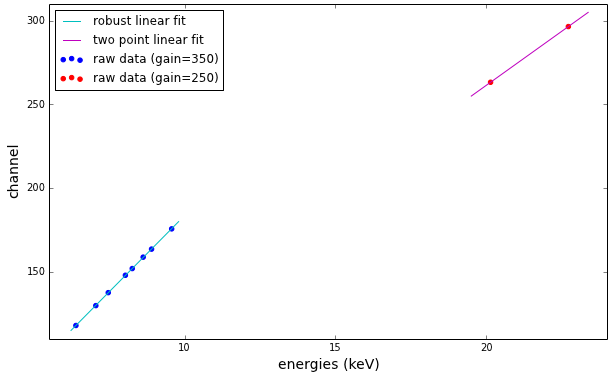
\includegraphics[width=0.8\textwidth]{calibration.png}
\caption{Two calibration curves made using least squares optimizations of linear functions to raw data at two different gain levels}
\label{calib}
\end{figure}

\newpage

Using these calibration curves to determine the energies of the peaks we then fit another linear function of the form,
\begin{equation}\label{linear_form}
[E_{k_\alpha}]^{1/2}=C(Z+S),
\end{equation}
where $E_{k_\alpha}$ is the energy of the $k_{\alpha}$ peak, $Z$ is the atomic number of the material, and both $C$ and $S$ are constants, to peak data. Following a least squares optimization of the constants $C$ and $S$ we find their values to be $10.20\pm0.05\times10^{-2}$ keV$^{1/2}$ and $-1.20\pm0.01$ respectively. Our value for $C$ matches up to the expected value of $10.10\pm0.05\times10^{-2}$ keV$^{1/2}$ while the measured values $S$ differs from the known, but approximate value of 1.This linear fit along with the $k_\alpha$ data used to create it are shown in Fig \ref{atomic}

\begin{figure}[h]
\centering
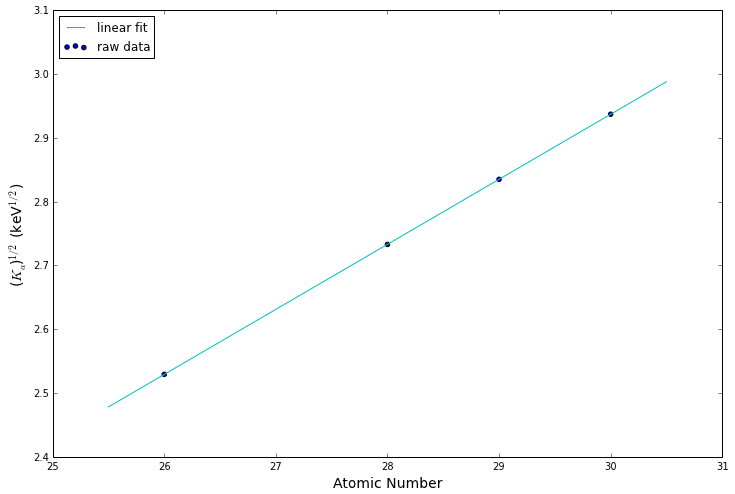
\includegraphics[width=0.8\textwidth]{atomic.png}
\caption{$k_\alpha$ peak data along with the linear fit defined by Eq \eqref{linear_form}}
\label{atomic}
\end{figure}

Two unknown materials were then analyzed. Their measured peaks were compared against a set of known element peaks to identify them. The measured peaks of the unknown $K_1$, $6.86\pm0.02$ keV and $8.12\pm0.02$ keV, were matched to the known values for the averaged $L_{\alpha1}$ and $L_{\alpha2}$ and the $L_{\beta2}$ peaks of Er$_{68}$ respectively.  The measured peaks of the unknown $K_2$, $7.45\pm0.02$ keV and $8.94\pm0.03$ keV, were matched to the known values for the average $L_{\alpha1}$ and $L_{\alpha2}$ and the $L_{\beta2}$ peaks of Yb$_{70}$ respectively. The measured peak of $15.70\pm0.04$ keV was unidentifiable and thus makes our identification of $K_2$ as Yb questionable.

\section{Conclusion}

In the end, after measure the constants $C$ and $S$ we found their values to be $10.20\pm0.05\times10^{-2}$ keV$^{1/2}$ and $-1.20\pm0.01$ respectively. Our value for $C$ matches up to the expected value of $10.10\pm0.05\times10^{-2}$ keV$^{1/2}$ while the measured values $S$ differs from the known, but approximate value of 1. The measured peaks of the unknown $K_1$, $6.86\pm0.02$ keV and $8.12\pm0.02$ keV, were matched to the known values for the averaged $L_{\alpha1}$ and $L_{\alpha2}$ and the $L_{\beta2}$ peaks of Er$_{68}$ respectively.  The measured peaks of the unknown $K_2$, $7.45\pm0.02$ keV and $8.94\pm0.03$ keV, were matched to the known values for the average $L_{\alpha1}$ and $L_{\alpha2}$ and the $L_{\beta2}$ peaks of Yb$_{70}$ respectively. The measured peak of $15.70\pm0.04$ keV was unidentifiable and thus makes our identification of $K_2$ as Yb questionable.

\end{document}
